% Harus dimuat terlebih dahulu, digunakan agar file PDF memiliki format karakter yang benar.
% Untuk informasi lebih lanjut, lihat https://ctan.org/pkg/cmap.
\RequirePackage{cmap}

% Format dokumen sebagai paper konferensi menggunakan aturan IEEEtran terbaru (v1.8b).
% Untuk informasi lebih lanjut, lihat http://www.michaelshell.org/tex/ieeetran/.
\documentclass[conference]{IEEEtran}[2015/08/26]

% Format encoding font dan input menjadi 8-bit UTF-8.
\usepackage[T1]{fontenc}
\usepackage[utf8]{inputenc}

% Format bahasa menjadi bahasa german dan inggris.
\usepackage[indonesian]{babel}

% Digunakan untuk tujuan demonstrasi.
\usepackage{mwe}

% Digunakan untuk menampilkan font dengan style yang lebih baik.
\usepackage[zerostyle=b,scaled=.75]{newtxtt}

% Digunakan untuk menampilkan tabel dengan style yang lebih baik.
\usepackage{booktabs}

% Digunakan untuk menampilkan gambar pada dokumen.
\usepackage{graphicx}

% Digunakan untuk menampilkan potongan kode.
\usepackage{listings}
\lstset{
  basicstyle=\ttfamily,
  columns=fixed,
  basewidth=.5em,
  xleftmargin=0.5cm,
  captionpos=b
}

% Digunakan agar backticks (`) dapat dirender pada PDF.
% Untuk informasi lebih lanjut, lihat https://tex.stackexchange.com/a/341057/9075.
\usepackage{upquote}

% Digunakan untuk menyeimbangkan bagian akhir dokumen dengan dua kolom.
\usepackage{balance}

% Digunakan untuk menampilkan pustaka.
\usepackage[square,comma,numbers,sort&compress]{natbib}

\usepackage{tabularx}
\usepackage{amsmath}
\usepackage{multirow}


% Mengubah format ukuran teks pada natbib.
\renewcommand{\bibfont}{\normalfont\footnotesize}

% Menambah nama penulis ketika menggunakan perintah \citet.
% Untuk informasi lebih lanjut, lihat https://tex.stackexchange.com/a/76075/9075.
\usepackage{etoolbox}
\makeatletter
\patchcmd{\NAT@test}{\else \NAT@nm}{\else \NAT@hyper@{\NAT@nm}}{}{}
\makeatother

\usepackage[hyphens]{url}
% Digunakan untuk menambah hyperlink pada referensi.
\usepackage{hyperref}

% Menonaktifkan warna dan bookmark pada hyperref.
\hypersetup{hidelinks,
  colorlinks=true,
  allcolors=black,
  pdfstartview=Fit,
  breaklinks=true
}

% Digunakan untuk membenarkan hyperref pada gambar.
\usepackage[all]{hypcap}

% Digunakan untuk menampilkan beberapa gambar
\usepackage[caption=false,font=footnotesize]{subfig}

\usepackage{stfloats}

\renewcommand\arraystretch{1.3}

% Tambahkan format tanda hubung yang benar di sini
\hyphenation{ }

\begin{document}

% Ubah kalimat berikut sesuai dengan judul penelitian.
\title{Deteksi Berita Palsu Otomatis Berbahasa Indonesia Menggunakan BERT}

% Ubah kalimat-kalimat berikut sesuai dengan nama, institusi, alamat dan kontak penulis.
\author{
  \IEEEauthorblockN{Reza Fuad Rachmadi}
  \IEEEauthorblockA{Departemen Teknik Komputer\\
    Fakultas Teknologi Elektro\\
    dan Informatika Cerdas\\
    Institut Teknologi Sepuluh Nopember\\
    Surabaya, Indonesia 60111\\
    fuad@te.its.ac.id}

  \and
  \IEEEauthorblockN{Mauridhi Hery Purnomo}
  \IEEEauthorblockA{Departemen Teknik Komputer\\
    Fakultas Teknologi Elektro\\
    dan Informatika Cerdas\\
    Institut Teknologi Sepuluh Nopember\\
    Surabaya, Indonesia 60111\\
    hery@ee.its.ac.id}

  \and
  \IEEEauthorblockN{Aufa  Nabil Amiri}
  \IEEEauthorblockA{Departemen Teknik Komputerr\\
    Fakultas Teknologi Elektro\\
    dan Informatika Cerdas\\
    Institut Teknologi Sepuluh Nopember\\
    Surabaya, Indonesia 60111\\
    aufa.17072@mhs.its.ac.id}
}

% Digunakan untuk menampilkan judul dan deskripsi penulis.
\maketitle

% Mengubah keterangan `Abstract` ke bahasa indonesia.
% Hapus bagian ini untuk mengembalikan ke format awal.
\renewcommand\abstractname{Abstrak}

\begin{abstract}

  % Ubah paragraf berikut sesuai dengan abstrak dari penelitian.
  Berita palsu atau yang biasa disebut hoaks adalah suatu yang hal yang sering melanda Indonesia. Dengan adanya sosial media, suatu berita palsu dapat memiliki tingkat penyebaran yang sangat luas. Selain itu, masyarakat Indonesia memiliki tingkat kecenderungan untuk menyebarkan berita palsu yang cukup tinggi. Sehingga, suatu metode pendeteksi berita palsu harus ada. Penelitian ini memanfaatkan algoritma BERT yang digunakan untuk mendeteksi apakah suatu berita adalah berita hoaks atau tidak secara otomatis. Dari suatu teks yang mentah, akan dilakukan tokenisasi sebelum akhirnya dimasukkan ke dalam algoritma BERT. Selanjutnya, keluaran dari BERT akan dijadikan sebagai inputan dari algoritma klasifikasi Linear Regression.  Barulah pada saat ini, kita bisa mendapatkan klasifikasi apakah suatu teks itu berupa berita hoaks atau tidak. Tujuan dari penelitian ini adalah untuk membuat sebuah model yang dapat digunakan untuk melakukan klasifikasi suatu teks apakah termasuk ke dalam berita hoaks atau tidak.

\end{abstract}

% Mengubah keterangan `Index terms` ke bahasa indonesia.
% Hapus bagian ini untuk mengembalikan ke format awal.
\renewcommand\IEEEkeywordsname{Kata kunci}

\begin{IEEEkeywords}

  % Ubah kata-kata berikut sesuai dengan kata kunci dari penelitian.
  BERT, Hoaks, Klasifikasi, Linear Regression

\end{IEEEkeywords}


% Ubah bagian berikut sesuai dengan konten-konten yang akan dimasukkan pada dokumen
% Ubah judul dan label berikut sesuai dengan yang diinginkan.
\section{Latar Belakang}
\label{sec:latarbelakang}

% Ubah paragraf-paragraf pada bagian ini sesuai dengan yang diinginkan.

Pesatnya perkembangan roket yang merupakan \lipsum[2-4]

Pembahasan pada paper ini dimulai dengan presentasi mengenai penelitian lain (Bagian \ref{sec:penelitianterkait}).
Kemudian dilanjutkan dengan penjelasan mengenai desain dan implementasi dari sistem yang dibuat (Bagian \ref{sec:desainimplementasi}).
Berdasarkan hal tersebut, kami menunjukkan lorem ipsum (Bagian \ref{sec:loremipsum}).
Terakhir, didapatkan kesimpulan dari penelitian yang telah dilakukan (Bagian \ref{sec:kesimpulan}).

%  % Ubah judul dan label berikut sesuai dengan yang diinginkan.
\section{Penelitian Terkait}
\label{sec:penelitianterkait}

Sudah terdapat beberapa penelitian yang pernah dilakukan oleh orang lain mengenai pendeteksi berita hoaks ini. Aggarway et al. pernah melakukan penelitian untuk membandingkan antara BERT, XGBoost dan LSTM untuk melakukan klasifikasi berita palsu berbahasa inggris. Dari penelitian tersebut didapatkan bahwa BERT memiliki tingkat akurasi yang lebih tinggi apabila dibandingkan dengan XGBoost dan LSTM \cite{bert_news_classi}. Bahad et al. melakukan penelitian yang membandingkan antara CNN, RNN, \textit{uni-directional} LSTM RNN dan \textit{bi-directional} LSTM RNN. Hasil dari penelitian tersebut menunjukkan bahwa penggunaan LSTM ditambah dengan \textit{attention} baik itu \textit{uni-directional} maupun \textit{bi-directional} memiliki tingkat akurasi yang lebih tinggi apabila dibandingkan dengan CNN atau RNN \cite{bahad_lstm}. Dari kedua penelitian tersebut, dapat diambil kesimpulan bahwa algoritma yang 'mengingat' atau mengetahui suatu konteks dalam teks akan memiliki tingkat akurasi yang lebih tinggi dibanding algoritma dengan pendekatan yang lain.

Untuk penelitian pendeteksi berita hoaks dengan berbahasa indonesia, terdapat beberapa penelitian yang pernah dilakukan seperti oleh Prasetijo et al. yang meneliti penggunaan SVM dan SGD untuk mendeteksi berita hoaks berbahasa indonesia. Penelitian tersebut berhasil membuat suatu model dengan tingkat akurasi sebesar 85\% \cite{prasetijo}. Penelitian lain yang dilakukan oleh Rahutomo et al. dengan menggunakan algoritma \textit{naive bayes} berhasil menghasilkan akurasi sebesar 80\% \cite{rahutomo}.

% Ubah judul dan label berikut sesuai dengan yang diinginkan.
\section{Desain dan Implementasi Sistem}
\label{sec:desainimplementasi}

% Ubah paragraf-paragraf pada bagian ini sesuai dengan yang diinginkan.

Pada cetak biru yang tertera pada Gambar \ref{fig:cetakbiru}. \lipsum[8]

% Contoh input gambar pada kolom.
\begin{figure} [ht]
  \centering
  % Ubah sesuai dengan nama file gambar dan ukuran yang akan digunakan.
  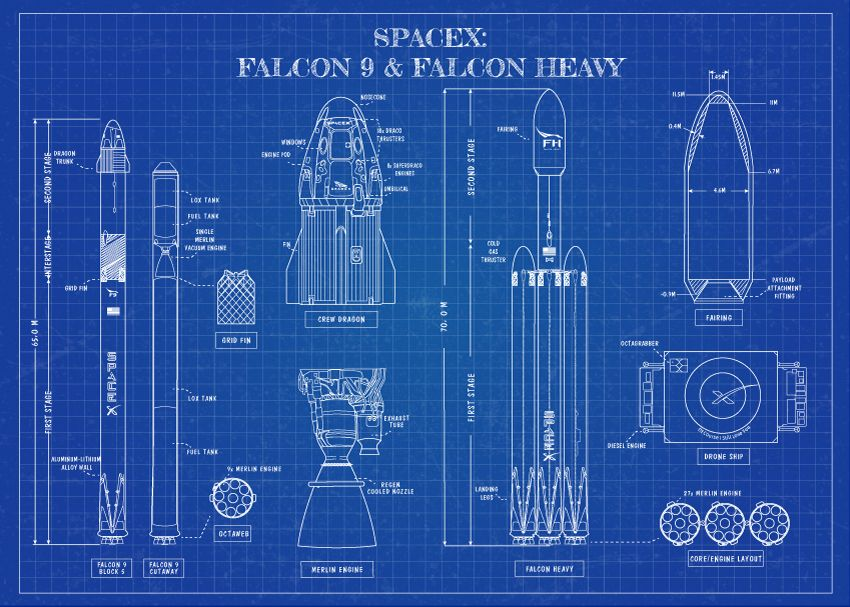
\includegraphics[width=0.4\textwidth]{gambar/cetakbiru.jpg}

  % Ubah sesuai dengan keterangan gambar yang diinginkan.
  \caption{Cetak biru roket yang akan diuji coba. \cite{cetakbiruspacex}}
  \label{fig:cetakbiru}
\end{figure}

\lipsum[9-11]

% Contoh pembuatan tabel.
\begin{table}
  \caption{Contoh tabel sederhana}
  \label{tab:tabelsederhana}
  \centering
  \begin{tabular}{lll}
    \toprule
    Heading1 & Heading2 & Heading3  \\
    \midrule
    One      & Two      & Three     \\
    Four     & Five     & Six       \\
    \bottomrule
  \end{tabular}
\end{table}

% Contoh pembuatan potongan kode.
\begin{lstlisting}[
  language=C++,
  caption={Program halo dunia.},
  label={lst:halodunia}
]
#include <iostream>

int main() {
    std::cout << "Halo Dunia!";
    return 0;
}
\end{lstlisting}

\lipsum[12]

% Contoh pembuatan daftar.
\begin{enumerate}
  \item \lipsum[13][1-4]
  \item \lipsum[13][5-8]
  \item \lipsum[13][9-12]
\end{enumerate}

\lipsum[14-15]

% Ubah judul dan label berikut sesuai dengan yang diinginkan.
\section{Hasil dan Pembahasan}
\label{sec:hasilpembahasan}

% Ubah bagian-bagian berikut dengan isi dari pengujian dan analisis
Pada penelitian ini dipaparkan hasil pengujian serta analisis yang dilakukan sesuai dengan desain sistem yang sudah dirancang pada bab sebelumnya. Dataset yang digunakan berasal dari \url{data.mendeley.com} ditambah dengan dataset yang berasal dari proses \textit{webcrawling} sendiri. Pengujian dilakukan dengan beberapa bagian sebagai berikut :

\begin{enumerate}[nolistsep]
    \item Pengujian Performa berdasar pada Penggalan Kata yang Diambil
    \item Pengujian Performa berdasarkan model BERT yang digunakan
    \item Pengujian Performa berdasarkan Pendekatan Cara \textit{Training}.
\end{enumerate}

Pada pengujian, masing - masing model menggunakan Google Collab dengan spesifikasi \textit{hardware} seperti yang dilampirkan pada tabel \ref{tab:specs_collab}

\begin{table}
    \caption{spesifikasi PC yang digunakan}
    \label{tab:specs_collab}
    \centering
    \begin{tabular}{|l|l|}
        \hline
        \textbf{Prosessor}            & 2 v-core Intel(R) Xeon(R) CPU @ 2.20GHz   \\ \hline
        \textbf{RAM}                  & Virtual Memory : 12GB                     \\ \hline
        \textit{\textbf{Storage}}     & SSD : 69GB                                \\ \hline
        \multirow{2}{*}{\textbf{GPU}} & Nvidia Tesla T4 16GB                      \\ \cline{2-2}
                                      & Nvidia K80 12GB                           \\ \hline
        \textbf{Sistem Operasi}       & Ubuntu 18.04.5 LTS (Bionic Beaver) 64-bit \\ \hline
    \end{tabular}
\end{table}

\subsection{Pengujian Performa berdasar pada Penggalan Kata yang Diambil}

Untuk saat ini, BERT hanya dapat memproses sebanyak 512 token sekaligus. Sehingga, untuk melakukan pemprosesan pada data dengan teks yang panjang, diperlukan pemotongan teks agar panjang teks menjadi sesuai.

Pengujian performa berdasar pada penggalan kata yang diambil ini bertujuan untuk mengetahui tingkat akurasi model BERT pada teks dengan cara pemotongan yang berbeda. Pembedaan ini dilakukan berdasarkan pada adanya berita yang menuliskan kesimpulan di awal, atau bisa juga menuliskan kesimpulan di akhir. Alternatif lain adalah mengambil sebagian teks di bagian awal dan mengambil sisanya di bagian akhir. Maka dari itu, dalam pengujian performa ini dilakukan dengan membagi teks pada beberapa cara memenggal kata, dengan rincian sebagai berikut :

\begin{enumerate}
    \item Mengambil bagian awal teks

          Terdapat beberapa ciri - ciri yang terdapat pada kebanyakan teks berita berbahasa Indonesia, salah satu dari ciri - ciri tersebut adalah menuliskan ringkasan berita pada paragraf awal kalimat. Format seperti ini biasanya cukup sering ditemui terutama pada berita yang memanfaatkan fitur halaman pada teks beritanya. Karenanya, pada jenis - jenis berita seperti ini, orang hanya perlu melihat beberapa kalimat awal untuk mengetahui apakah bahwa berita tersebut valid dan dapat dipercaya.

    \item Mengambil bagian akhir teks

          Mirip seperti pengujian dengan mengambil bagian awal teks, terdapat ciri - ciri lain yang biasanya terdapat pada teks berita berbahasa Indonesia adalah adanya kesimpulan pada bagian akhir teks berita. Sehingga, setelah isi berita yang biasanya dibahas cukup dalam, pembaca dapat mengetahui bagaimana dan apa hubungan setiap informasi yang disajikan dengan peristiwa yang sedang dibahas dalam berita.

    \item Mengambil 129 token dari bagian awal teks dan 383 token dari bagian akhir teks

          Pengujian ini berdasarkan pada penelitian Chi Sun et al. yang menemukan bahwa dengan strategi pengambilan teks yang dibagi dua seperti ini akan dapat memberikan nilai akurasi yang lebih baik apabila dibandingkan dengan mengambil hanya di bagian awal maupun di bagian akhir saja \cite{sun2019fine}. Alasan dari penyebab lebih tingginya akurasi adalah karena dengan mengambil sebagian di awal maka sebagian dari ringkasan berita akan didapatkan, sedangkan mengambil sebagian di akhir adalah agar kesimpulan berita juga masuk ke dalam proses \textit{training}. Namun, pengujian tersebut dilakukan pada dataset teks berita berbahasa Inggris sehingga masih harus dilakukan pengujian lagi pada dataset teks berita berbahasa Indonesia.

\end{enumerate}

Dari total data yang berjumlah 1621 data, akan diambil 18\% nya sebagai dataset pengujian, sehingga berjumlah 292 dataset sebagai pengujian. Parameter pada pengujian untuk \textit{training} di atur agar sama untuk setiap pengujian, \textit{epoch} sebesar 7, \textit{leearning rate} sebesar 2e-5, dan \textit{epsilon} sebesar 1e-8, hal yang sama juga dilakukan pada model, pengujian ini menggunakan model BERT yang telah di-\textit{pre-trained} oleh Indobert. Untuk lebih jelasnya, silahkan lihat Tabel \ref{tab: truncate_param} yang berisi rincian parameter dan model yang digunakan untuk proses \textit{training}.

\begin{table}
    \caption{Konfigurasi Parameter Untuk Pengujian berdasarkan Pemotongan Kata}
    \label{tab: truncate_param}
    \centering
    \begin{tabular}{|l|l|}
        \hline
        \textit{\textbf{epoch}}          & 3                              \\ \hline
        \textit{\textbf{learning rates}} & 2e-5                           \\ \hline
        \textit{\textbf{epsilon}}        & 1e-4                           \\ \hline
        \textbf{model}                   & indobenchmark/indobert-base-p1 \\ \hline
    \end{tabular}
\end{table}

Keluaran dari model akan dibandingkan dengan label pada dataset, yang kemudian akan dihitung untuk menghasilkan \textit{confusion matrix}, \textit{recall, precision, accuracy} dan \textit{f1-score} sesuai dengan rumus yang telah dijelaskan sebelumnya.

\begin{table}
    \centering
    \caption{Performa pada pengujian berdasar pada lokasi pemotongan kata}
    \label{tab: truncate_result}
    \begin{tabular}{|p{.12\textwidth}|l|l|l|l|}
        \hline
        \textbf{lokasi pemotongan}      & \textit{\textbf{recall}} & \textit{\textbf{precision}} & \textit{\textbf{f1-score}} & \textit{\textbf{accuracy}} \\ \hline
        awal                            & \textbf{89\%}            & \textbf{90\%}               & \textbf{89\%}              & \textbf{89\%}              \\ \hline
        akhir                           & 88\%                     & 85\%                        & 86\%                       & 86\%                       \\ \hline
        gabungan (129 awal + 383 akhir) & 88\%                     & 88\%                        & 88\%                       & 87\%                       \\ \hline
    \end{tabular}
\end{table}

Seperti bisa dilihat pada tabel \ref{tab: truncate_result}, metode pemotongan teks dengan hanya mengambil bagian awal saja memiliki tingkat akurasi yang paling tinggi dan memiliki nilai \textit{recall} dan \textit{precision} yang seimbang. Hal ini berbeda dengan apabila dilakukan pemotongan pada bagian akhir teks yang menunjukkan ada kemungkinan lebih besar bagi model untuk mengklasifikasi suatu teks berita termasuk ke dalam berita palsu. Metode pemotongan yang menggabungkan 129 token dari awal dan 383 token dari bagian akhir teks memiliki rasio nilai \textit{recall} dan \textit{precision} yang bagus juga sama seperti rasio nilai pada pemotongan pada bagian awal teks, namun, secara isi nilai masih kalah.

\subsection{Pengujian Performa berdasarkan model BERT yang digunakan}

Terdapat banyak sekali model BERT yang sudah dibuat oleh berbagai orang di internet, ada model yang memiliki kemampuan \textit{multilanguage} sehingga bisa digunakan di berbagai bahasa sekaligus, namun kebanyakan model yang beredar adalah model yang menggunakan bahasa yang spesifik. Hal ini karena waktu \textit{pre-training} yang lebih singkat karena dataset yang lebih sedikit apabila dibandingkan model dengan kemampuan \textit{multilanguage} dan karena waktu \textit{pre-training} lebih sedikit, maka sumber daya yang digunakan juga menjadi lebih sedikit. Selain itu, dan hal ini adalah yang paling penting, hasil akurasi dari model yang hanya menggunakan 1 bahasa memiliki tingkat akurasi yang lebih tinggi apabila dibandingkan dengan model dengan banyak bahasa sekaligus. Maka dari itu, kami menggunakan beberapa model dengan rincian sebagai berikut :

\begin{enumerate}
    \item bert-base-bahasa-standard-case

          Merupakan model BERT yang dibuat oleh

\end{enumerate}

Untuk model BERT yang menggunakan hanya bahasa Indonesia, terdapat 2 model yang bisa ditemukan pada waktu buku ini ditulis. Yang pertama dibuat oleh Bryan Wilie et al., sebagai bagian dari pengujian \textit{benchmark} berbahasa Indonesia dengan model BERT yang dilatih khusus dengan dataset berbahasa Indonesia juga \cite{wilie2020indonlu}. Hasil dari pengujian tersebut adalah model yang mereka buat berhasil memperoleh tingkat akurasi yang lebih tinggi apabila dibandingkan dengan model - model lain seperti XLM atau mBERT yang memiliki dukungan untuk melakukan tugas prediksi dengan banyak bahasa sekaligus \cite{wilie2020indonlu}. Model kedua dibuat oleh Candra Wirawan dengan melatih model pada 520MB data berasal dari Wikipedia Indonesia dan 1GB data berasal dari teks berita Indonesia. Sayangnya, tidak ada informasi lebih lanjut pada model ini selain data yang dipakai untuk \textit{pre-training}.

Selain model BERT yang hanya berisi bahasa Indonesia, kami juga melakukan percobaan pada model BERT yang mendukung \textit{multilanguage} dan model BERT yang hanya berisi bahasa Melayu. Bahasa Melayu dipilih karena kedekatan \textit{grammar} dan konteks dengan susunan kata berbahasa Indonesia. Untuk model yang mendukung \textit{multilanguage} kami menggunakan varian \textit{official} yang dibuat oleh Google, yaitu model \texttt{bert-multilingual-uncased} yang sudah mendukung 104 bahasa yang berasal dari Wikipedia. Sedangkan untuk model dengan bahasa Melayu, kami menggunakan model \texttt{bert-base-bahasa-standard-cased} yang sudah dilatih di beberapa sumber seperti Wikipedia, Wattpad, Berita, Sosial Media dan masih banyak lagi \cite{Malaya}

\begin{table}
    \centering
    \caption{Konfigurasi yang digunakan oleh model BERT yang digunakan}
    \label{tab:multi_bert_config}
    \begin{tabular}{|p{.5\linewidth}|c|l|p{.12\linewidth} |}
        \hline
        Model                          & epoch & dropout & learning rates \\ \hline
        bert-base-bahasa-standard-case & 4     & 0.2     & 2e-5           \\ \hline
        bert-base-multilingual-uncased & 4     & 0.2     & 2e-5           \\ \hline
        indobert-base-p1               & 3     & 0.1     & 2e-5           \\ \hline
        bert-base-indonesian-522M      & 3     & 0.1     & 2e-5           \\ \hline
        bert-base-indonesian-1.5G      & 3     & 0.2     & 2e-5           \\ \hline
    \end{tabular}
\end{table}

Untuk melakukan \textit{training}, sebelumnya kami mengatur konfigurasi yang akan digunakan oleh model BERT yang sudah disiapkan. Terdapat beberapa perbedaan pada konfigurasi seperti jumlah \textit{epoch} dan jumlah \textit{dropout}. Hal ini karena pada beberapa model, apabila menggunakan konfigurasi \textit{default} akan terjadi \textit{overfit} yang cukup parah.

\begin{table}
    \centering
    \caption{Tingkat Akurasi dari seluruh model BERT yang digunakan}
    \label{tab:model_bert_result}
    \begin{tabular}{|l|l|l|l|l|p{.12\linewidth}|}
        \hline
        \textbf{model} & \textit{\textbf{recall}} & \textit{\textbf{precision}} & \textit{\textbf{f1-score}} & \textit{\textbf{accuracy}} & \textbf{avg. training time} \\ \hline
        bert-bahasa    & 89\%                     & 82\%                        & 85\%                       & 85\%                       & 03:43                       \\ \hline
        bert-base      & \textbf{97\%}            & 75\%                        & 85\%                       & 86\%                       & 02:07                       \\ \hline
        indobert       & 89\%                     & \textbf{90\%}               & \textbf{89\%}              & \textbf{89\%}              & 02:05                       \\ \hline
        cahya-522M     & 88\%                     & 80\%                        & 84\%                       & 84\%                       & \textbf{02:03}              \\ \hline
        cahya-1.5G     & 93\%                     & 80\%                        & 86\%                       & 87\%                       & 02:08                       \\ \hline
    \end{tabular}
\end{table}
% Ubah judul dan label berikut sesuai dengan yang diinginkan.
\section{Kesimpulan}
\label{sec:kesimpulan}

% Ubah paragraf-paragraf pada bagian ini sesuai dengan yang diinginkan.

\lipsum[21-23]


% Menampilkan daftar pustaka dengan format IEEE
\bibliographystyle{IEEEtranN}
\bibliography{pustaka/pustaka.bib}

% Menyeimbangkan bagian akhir di kedua kolom
\balance

%\clearpage

%\section*{Appendix}
\label{sec:appendix}

\begin{figure}[h]
    \begin{center}
        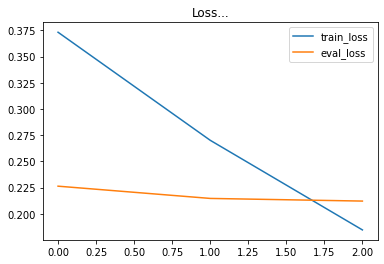
\includegraphics[width= 0.9\linewidth]{gambar/loss_concat_awal.png}
        \caption{Nilai \textit{Loss} saat Pengujian dengan Mengambil Bagian Awal Teks}
        \label{fig: loss_const_awal}
    \end{center}
\end{figure}

\begin{figure}[h]
    \begin{center}
        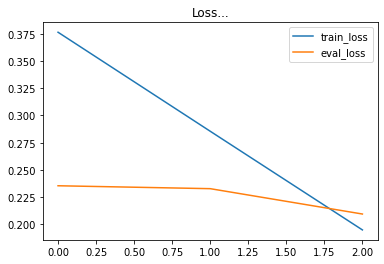
\includegraphics[width= 0.9\linewidth]{gambar/loss_concat_tengah.png}
        \caption{Nilai \textit{Loss} saat Pengujian dengan Mengambil Bagian Tengah Teks}
        \label{fig: loss_const_tengah}
    \end{center}
\end{figure}

\begin{figure}[h]
    \begin{center}
        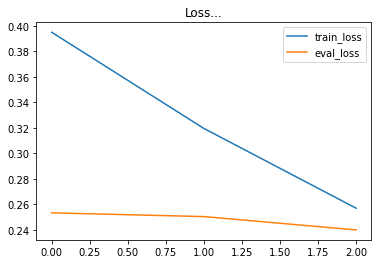
\includegraphics[width= 0.9\linewidth]{gambar/loss_bert_bahasa.png}
        \caption{Nilai \textit{Loss} saat Pengujian dengan model \textit{bert-bahasa}}
        \label{fig: loss_bert_bahasa}
    \end{center}
\end{figure}

\begin{figure}[h]
    \begin{center}
        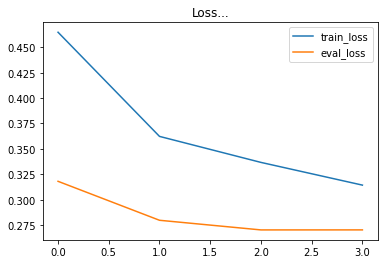
\includegraphics[width= 0.9\linewidth]{gambar/loss_bert_multilingual.png}
        \caption{Nilai \textit{Loss} saat Pengujian dengan model \textit{bert-base}}
        \label{fig: loss_bert_multilingual}
    \end{center}
\end{figure}

\begin{figure}[h]
    \begin{center}
        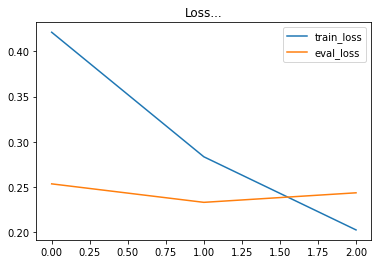
\includegraphics[width= 0.9\linewidth]{gambar/loss_cahya_bert_522.png}
        \caption{Nilai \textit{Loss} saat Pengujian dengan model \textit{cahya-522M}}
        \label{fig: loss_bert_cahya522}
    \end{center}
\end{figure}

\begin{figure}[h]
    \begin{center}
        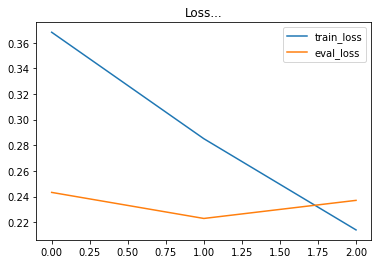
\includegraphics[width= 0.9\linewidth]{gambar/loss_cahya_bert_1,5.png}
        \caption{Nilai \textit{Loss} saat Pengujian dengan model \textit{cahya-1.5G}}
        \label{fig: loss_cahya1.5}
    \end{center}
\end{figure}

\begin{figure}[h]
    \begin{center}
        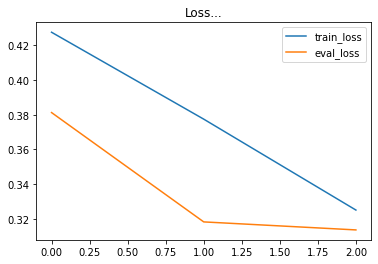
\includegraphics[width= 0.9\linewidth]{gambar/loss_roberta522.png}
        \caption{Nilai \textit{Loss} pada model ROBERTA}
        \label{fig: loss_roberta}
    \end{center}
\end{figure}


\begin{figure}[h]
    \begin{center}
        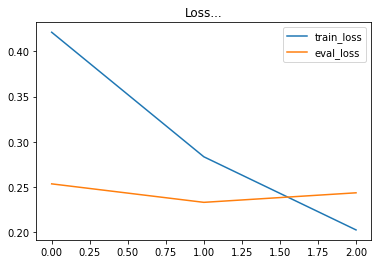
\includegraphics[width= 0.9\linewidth]{gambar/loss_cahya_bert_522.png}
        \caption{Nilai \textit{Loss} pada model BERT}
        \label{fig: loss_bert}
    \end{center}
\end{figure}

\begin{figure}[h]
    \begin{center}
        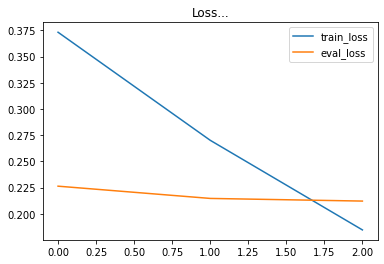
\includegraphics[width= 0.9\linewidth]{gambar/loss_concat_awal.png}
        \caption{Nilai \textit{Loss} saat Pengujian dengan model \textit{indobert}}
        \label{fig: loss_bert_indobert}
    \end{center}
\end{figure}


\end{document}
